%Die Angabe des schlauen Spruchs auf diesem Wege funtioniert nur,
%wenn keine Änderung des Kapitels mittels den in preambel/chapterheads.tex
%vorgeschlagenen Möglichkeiten durchgeführt wurde.
\chapter{Problem Definition and Feature Selection}
\label{chap:chapter4}
%\vspace{-3cm}
%\vspace{2cm}

There are a number of methods to separate permanent faults from non-recurring faults as explained in the section~\ref{sec:secfc}. However available techniques do not separate faults as permanent, transient and intermittent. This is of particular importance from the point of view of reducing yield loss, by including chips which showed only transient faults. Also, if faults can be categorized into permanent transient or intermittent, then it gives additional information to the designer about the underlying fault mechanism, so that additional optimization of yield can be achieved. 

The yield can be improved by taking the rejected chips, and analyzing them further by running tests again multiple ($TestRuns$) times, and decide on what type of fault caused the failure during the test. These chips that showed a non-critical fault can still be included in the final yield. However an incorrect analysis would result in degradation of product quality. Hence, the classifier should be as accurate as possible.

The criticality of a fault is an abstract concept and it is defined by the application domain of the final product. Sometimes the user is more interested in optimizing the yield for quality, he would then wish to reject all chips with a slightest possibility of intermittent failure. In this case the classifier should be optimized for classifying intermittent faults more accurately. However, this would happen at an expense of healthy chips which showed intermittent failures result in yield loss. On the other hand, if the user wants to optimize for yield, classifier should be tuned to classify transient faults more accurately, which can impact product quality as more intermittents would be classified inaccurately. The classifier to be designed needs to take this fact in consideration and should provide the user with the functionality to find a suitable trade-off between the amount of yield and its quality.

The classification approaches explained in section~\ref{sec:secfc} are mostly rule or heuristic based (e.g. the threshold value in $\alpha$-counting techniques). Generally speaking, when an intermittent fault occurs in a system, its activation rate is higher than the transient fault rate \cite{Bondavalli2000}. However, as systems are moving to lower technology nodes, transient faults are also on the rise, as explained in section~\ref{sec:secft}. Hence with traditional techniques, it becomes difficult to separate transients from intermittents , as the fault rates for these two types of faults become close to each other. Hence an elaborate analysis is required to update these rules for every product and technology. Hence, the classifier to be designed should also focus on building a universal model, which can classify faults irrespective of the product and technology.

To summarize, we need an automated and adaptive approach which is independent on the product and the technology, and that can classify faults as intermittent, transient and permanent accurately. 

\section{Machine learning approach for fault classification}

Machine learning has been used in a wide variety of classification applications with a reasonable accuracy \cite{Pang2002,Nguyen2008,Sebastiani2002, Kotsiantis2007}. As explained in chapter~\ref{chap:chapter3}, machine learning is used when it is not practical to arrive at rules by looking at the data. Machine learning algorithms can be implemented as a \enquote{black-box} approach for classification and all the user needs to do is adjust a few parameters, depending on machine learning algorithm used. Even parameter searching can be automated and user can fine-tune them for further improvement in accuracy \cite{Hsu2003, Castillo2000}. This makes machine learning a practical and automated approach when large amount of data is available.

Once a feature set is fixed and the learning parameters are decided, machine learning algorithms analyze the data to set up a classification model. When a technology node is updated, one might have to change the database and train the algorithm again, but the training algorithm takes care of the changed feature space and builds a new classification model accordingly, making machine learning approaches adaptive.

Figure~\ref{fig:mlsteps} explains the basic steps for classification using machine learning methods.

\begin{figure}[h]
  \begin{center}
    \captionsetup{justification=centering}
    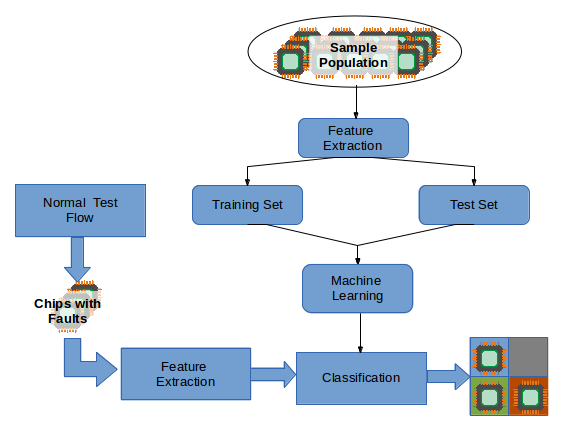
\includegraphics[scale=0.65]{figures/mlsteps.png}
    \caption{Classification of VLSI chips using machine learning}
    \label{fig:mlsteps}
  \end{center}
\end{figure}

First step in designing a machine learning system for classification is to decide on features, which can be efficiently classify the data. Selection of proper features has the most impact in accuracy of any classifier \cite{Michie1994}. This, along with design of methods to extract features from input data is explained in section~\ref{sec:secfs} of this chapter. Selection machine learning algorithm is to be used is explained in the last section of this chapter. Next step is to generate sample population, covered in the next chapter.

\section{Feature Selection}
\label{sec:secfs}
To begin with the feature selection, it is important to take a look at all the behavioral characteristics of different types of faults, as covered in chapter~\ref{chap:chapter2}. Table~\ref{tab:charfaults} summarizes all important characteristics to be considered for selection of features. Rest of the section describes features that were selected and algorithms for extraction of those features.

{%
\newcommand{\mc}[3]{\multicolumn{#1}{#2}{#3}}
\begin{table}[H]
 \begin{center}
  \captionsetup{justification=centering}
  \begin{tabular}{lp{4cm}p{4cm}p{4cm}}
	\hline
    \mc{1}{c}{\textbf{Characteristic}} & \mc{1}{c}{\textbf{Permanent faults}} & \mc{1}{c}{\textbf{Intermittent faults}} & \mc{1}{c}{\textbf{Transient faults}}\\ \hline
    Affected outputs & Affects same set of output pins & Affects same set of output pins & Affects any of primary outputs\\
    Reproducibility & Reproducible for same test vector & Sometimes reproducible for same test vector depending upon the fault activation rate & Not reproducible\\
    Location on chip & Fixed to a fault location & Fixed to a fault location & Can affect any location on chip\\
    Fault behavior & Deterministic & Non-deterministic & Non-deterministic \\ \hline
  \end{tabular}
  \caption{Characteristics of faults in VLSI systems}
  \label{tab:charfaults}
 \end{center}
\end{table}
}%

\subsection{Reproducibility of fault}
The reproducibility of a fault pattern during multiple test runs is defined as the maximum number of maximum occurrences of same faulty output pattern for a fixed input pattern, and it is denoted by $\epsilon$.

Let the $P$ be the test pattern set, $OP_{i,j}$ be output pattern and $REF_i$ be the reference output at input $i$ and test run $j$ then,

\[\begin{array}{lp{10cm}} 
\epsilon = \max\limits_{i \in P}{\left\{\max\limits_{j \in TestRuns} \left\{\sum\limits_{k \in TestRuns} 1 \cdot e_{ijk}\right\} \right\}} & \\
\mbox{where;} &\\
e_{ij} = 1 & \mbox{when $OP_{ij},OP_{ik} \neq REF_i$, $OP_{ij} = REF_{ik}$,}\\
&\mbox{$j\neq k$ and $i \in P$, $j,k \in TestRuns$ }\\
e_{ij} = 0 & \mbox{otherwise}
\end{array} \]

\begin{figure}[h]
  \begin{center}
    \captionsetup{justification=centering}
    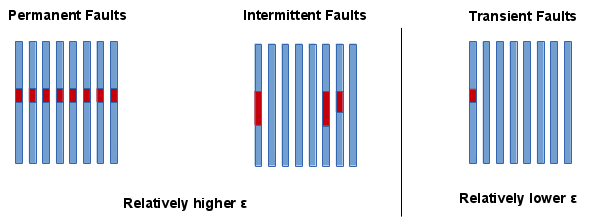
\includegraphics[scale=0.65]{figures/epsilon.png}
    \caption{Expected behavior of $\epsilon$ for different faults}
    \label{fig:epsilon}
  \end{center}
\end{figure}

Algorithm~\ref{alg:epsilon} explains extraction of $\epsilon$. It takes the expected and actual output patterns as inputs. It then checks if any of output patterns was faulty and it calculates maximum occurrences of every faulty pattern for given input pattern and stores in into array. Final value of $\epsilon$ is maximum value of in this array.

\begin{algorithm}[H]
  \caption{Algorithm to evaluate $\epsilon$}
  \label{alg:epsilon}
  \begin{algorithmic}
 \Procedure{ComputeEpsilon}{Expected output pattern array (EX), Observed output pattern array for all test runs (OP)}
 \State $\epsilon$[size(EX)] $\leftarrow$ 0\;
 \State Index $\leftarrow$ 0\;
 \While{Index $<$ size(EX)}
  \If{EX[Index] $\neq$ any pattern of OP[Index][]}
   \State $\epsilon$[Index] $\leftarrow$ max(\Call{SimilarFaultyPatterns}{OP[Index][]})\;
  \Else
   \State $\epsilon$[Index] $\leftarrow$ 0\;
  \EndIf
  \State Index++\;
 \EndWhile
 \State$\epsilon$ $\leftarrow$ max($\epsilon$[])\;
 \State \Return $\epsilon$\;
 \EndProcedure
 \end{algorithmic}
\end{algorithm}

Figure~\ref{fig:epsilon} shows expected behavior of $\epsilon$ for different fault types. Permanent faults are repeatable and value of $\epsilon$ is expected to be equal to the number of test runs for these type of faults. Intermittent faults occur at higher rate than that of transients for a fixed input pattern, hence they are also expected to have somewhat higher value than transient faults. Figure~\ref{fig:epsilonp45k} shows actual values of $\epsilon$ for a simple circuit (p45k). It should be noted that in this figure, some of the intermittents (marked in red) also have the value of $\epsilon = 1$, which is not clearly visible due to resolution constraints and relatively large amount of data.

\begin{figure}[h]
  \begin{center}
    \captionsetup{justification=centering}
    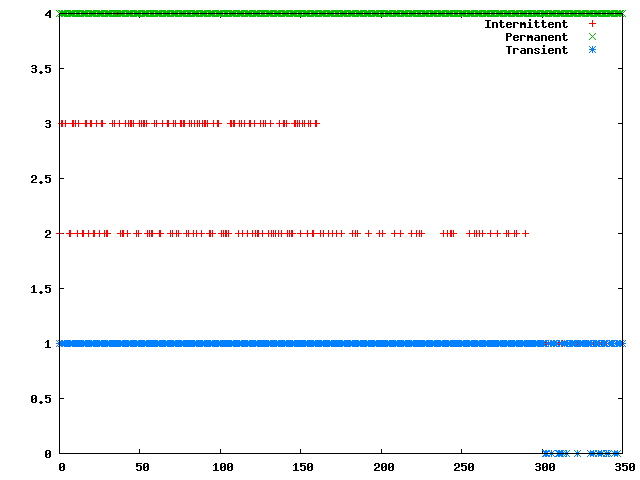
\includegraphics[scale=0.35]{figures/epsilonp45k.png}
    \caption{Plot of $\epsilon$ for p45k}
    \label{fig:epsilonp45k}
  \end{center}
\end{figure}

\subsection{Resemblance of erroneous output patterns}
The resemblance of erroneous output patterns is defined in terms of the hamming distance between a set of erroneous output patterns obtained during multiple test runs, for the same input test pattern in a test set. The \emph{Hamming Distance} of a set is evaluated as the maximum of number of positions in which the output patterns differ, pairwise. It is denoted using notation $\delta_H$, subscript $H$ stands for \enquote{horizontal}, denoting the orientation of calculation of the hamming distance. If all output patterns for an input test pattern are correct then the hamming distance and hence the value of $\delta_H$ would be zero.

Let the $P$ be the test pattern set, $OP_{i,j}$ be output pattern and $REF_i$ be the reference output at input $i$ and test run $j$ then,

\[
\delta_H = \max\limits_{i\in P} \left\{HammingDistance 
\left\{OP_{ij} | OP_{ij} \neq REF_i \forall j \in TestRuns\right\} 
\right\} 
\]

\begin{figure}[h]
  \begin{center}
    \captionsetup{justification=centering}
    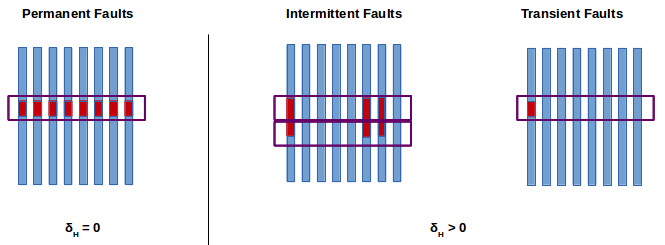
\includegraphics[scale=0.65]{figures/deltah.png}
    \caption{Expected behavior of $\delta_H$ for different faults}
    \label{fig:deltah}
  \end{center}
\end{figure}

Algorithm~\ref{alg:deltah} explains extraction of $\delta_H$. It takes the expected and actual output patterns as inputs. It then checks if any of output patterns is faulty, to save some computational efforts. If  any of output patterns is faulty, it calculates the value of $\delta_H$ and stores it in an array against the corresponding index of the input pattern. The final value of $\delta_H$ is maximum value of $\delta_H$ in this array. 

\begin{algorithm}[H]
  \caption{Algorithm to evaluate $\delta_H$}
  \label{alg:deltah}
  \begin{algorithmic}
 \Procedure{ComputeDeltaH}{Expected output pattern array (EX),Observed output pattern array for all test runs (OP)}
 \State $\delta_H$[size(EX)] $\leftarrow$ 0\;
 \State Index $\leftarrow$ 0\;
 \While{Index $<$ size(EX)}
  \If{EX[Index] $\neq$ any pattern of OP[Index][]}
   \State $\delta_H$[Index] $\leftarrow$ \Call{HammingDistance}{OP[Index][]}\;
  \Else
   \State $\delta_H$[Index] $\leftarrow$ 0\;
  \EndIf
  \State Index++\;
 \EndWhile
 \State$\delta_H$ $\leftarrow$ max($\delta_H$[])\;
 \State \Return $\delta_H$\;
 \EndProcedure
 \end{algorithmic}
\end{algorithm}

Figure~\ref{fig:deltah} shows expected behavior of $\delta_H$ for different fault types. Permanent faults repeat with same faulty output pattern and value of $\delta_H$ is expected to be zero. Intermittent faults, even though fail with same faulty output, are not repeatable and hence are expected to have a $\delta_H$ value other than zero. Transient fail randomly at random output locations and hence are expected to have higher $\delta_H$ value. Figure~\ref{fig:deltahp45k} shows actual values of $\delta_H$ for a simple circuit (p45k).

\begin{figure}[h]
  \begin{center}
    \captionsetup{justification=centering}
    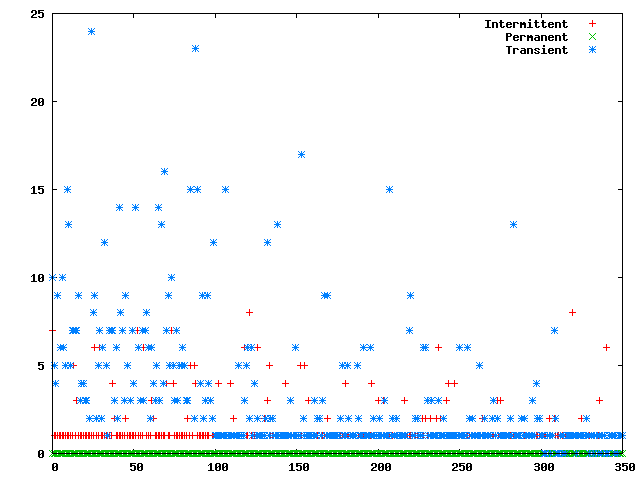
\includegraphics[scale=0.35]{figures/deltahp45k.png}
    \caption{Plot of $\delta_H$ for p45k}
    \label{fig:deltahp45k}
  \end{center}
\end{figure}

\subsection{Resemblance of erroneous primary outputs}
Resemblance of erroneous primary outputs is defined as hamming distance between primary output locations, that showed a faulty behavior at least once for a respective test run. This quantity is denoted by $\delta_V$, subscript $V$ denoting \emph{vertical} collapsing of all faulty primary outputs for a test run, before evaluating hamming distance.

Let the $P$ be the test pattern set, $OP_{i,j}$ be output pattern and $REF_i$ be the reference output at input $i$ and test run $j$, The dirty pins are marked as a set $M_j$ for every test run $j$ as,

\[M_j = \{M_{j0}, M_{j1} \ldots M_{jn}\}\]

where $n$ is number of Primary Outputs. An element of this set $M_{jl},$ $0\leq l \leq n$ has value 1 if that PO showed faulty behavior at least once during the test run. This value is 0 otherwise.

$\delta_V$ is calculated as,

\[
\begin{array}{lp{10cm}} 
\delta_V = HammingDistance \{ M_j \} & \mbox{$\forall j \in TestRuns$}
\end{array} 
\]

Algorithm~\ref{alg:deltav} explains extraction of $\delta_V$ using the method above.

\begin{algorithm}[H]
  \caption{Algorithm to evaluate $\delta_V$}
  \label{alg:deltav}
  \begin{algorithmic}
 \Procedure{ComputeDeltaV}{Expected output pattern array (EX),Observed output pattern array for all test runs (OP)}
 \State $\delta_V$[TotalRuns] $\leftarrow$ 0\;
 \State CurrentRun $\leftarrow$ 0\;
 \While{CurrentRun $<$ TotalRuns}
  \State Index $\leftarrow$ 0\;
  \While{Index $<$ size(EX)}
	\State ExpectedOutput $\leftarrow$ EX[Index]\;
	\State ActualOutput $\leftarrow$ OP[Index][CurrentRun]\;
   \State Iterator $\leftarrow$ 0\;
	\While{Iterator $<$ length(ExpectedOutput)}
		\If{ExpectedOutput.CharAt(Iterator) $\neq$ ActualOutput.CharAt(Iterator)}
		 \State $\delta_V$[CurrentRun].CharAt(Iterator) $\leftarrow$ 1\;
		\Else
		 \State $\delta_V$[CurrentRun].CharAt(Iterator) $\leftarrow$ 0\;
		\EndIf
		\State Iterator++\;
		\EndWhile
	\State Index++\;
  \EndWhile
 \State CurrentRun++\;
 \EndWhile
 \State $\delta_V$ $\leftarrow$ \Call{HammingDistance}{$\delta_V$[]}\;
 \State \Return $\delta_V$\;
 \EndProcedure
 \end{algorithmic}
\end{algorithm}

It is expected that value of $\delta_V$ is low in case of permanent and intermittent faults, as these faults manifest into failures at fixed set of output pins. In contrast, transient faults do not have a fixed set of outputs that it affects,resulting in high expected value of $\delta_V$.  Figure~\ref{fig:deltavp45k} shows actual values of $\delta_V$ for a simple circuit (p45k).

\begin{figure}[h]
  \begin{center}
    \captionsetup{justification=centering}
    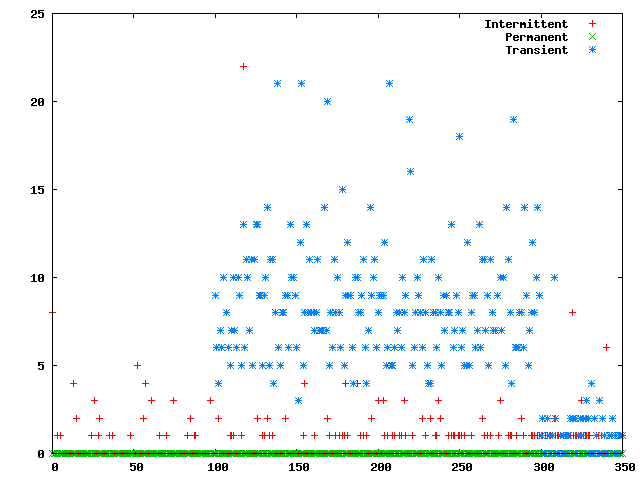
\includegraphics[scale=0.35]{figures/deltavp45k.png}
    \caption{Plot of $\delta_V$ for p45k}
    \label{fig:deltavp45k}
  \end{center}
\end{figure}

\subsection{Diagnostic features}
Diagnostic features from section~\ref{sec:secfd} are also considered as features for learning algorithm. Diagnostic data also provides information about fault present in circuit. A short summery of fault models and observed behavior for diagnostic parameters is summarized in table~\ref{tab:diagparam} \cite{Holst2009}.

\begin{table}[h]
\captionsetup{justification=centering}

\begin{tabular}{p{2cm}p{2.5cm}p{2.5cm}p{2.5cm}p{2.5cm}}
\hline
Fault type   & \multicolumn{1}{c}{$\sigma$}                              & \multicolumn{1}{c}{$\iota$}                           & \multicolumn{1}{c}{$\tau$}                            & \multicolumn{1}{c}{$\gamma$}                                                   \\ \hline
Permanent    & \textgreater0, same sigma values in all of the test runs. & \textgreater0, only with transient noise, otherwise 0 & \textgreater0, only with transient noise, otherwise 0 & \textgreater0, only for delay fault model, same values in all of the test runs \\
Intermittent & \textgreater0, low as compared to permanent faults        & \textgreater0, higher as compared to permanent faults & \textgreater0, only with transient noise, otherwise 0 & 0                                                                              \\
Transient    & \textgreater0, varies on every test run                     & \textgreater0, varies on every test run                 & \textgreater0, varies on every test run                 & \textgreater0, varies on every test run                                         \\
\hline
\end{tabular}

\caption{Expected evidence values for various fault types}
\label{tab:diagparam}
\end{table}


In this work it is assumed that at most only a single intermittent or permanent fault is active in the circuit with or without some transient noise (Refer section~\ref{sec:gsp:assumptions}). Most of the permanent faults can be modeled as a single stuck-at, single conditional stuck-at or a delay faults. Transient faults can be modeled as conditional stuck-at faults, at multiple fault sites as the do not have a fixed location on chip and some deterministic probability function can be used as trigging condition. Similarly intermittent faults can be modeled as single conditional stuck-at faults. Hence a combination of values of the parameters can be used to deduce which type of fault might exist on the chip.

Furthermore, the standard deviation of the evidence parameters is expected to be around zero for permanent faults, as once they are detected then they always be detected using the same test pattern set. Hence as standard deviations of evidence based features convey some information about fault class, they are also considered as features for learning. Figure~\ref{fig:sdevidance} shows actual values of standard deviation of evidence based features for a simple circuit (p45k).

\begin{figure}
        \centering
			\captionsetup{justification=centering}
        \begin{subfigure}[h]{0.45\linewidth}
                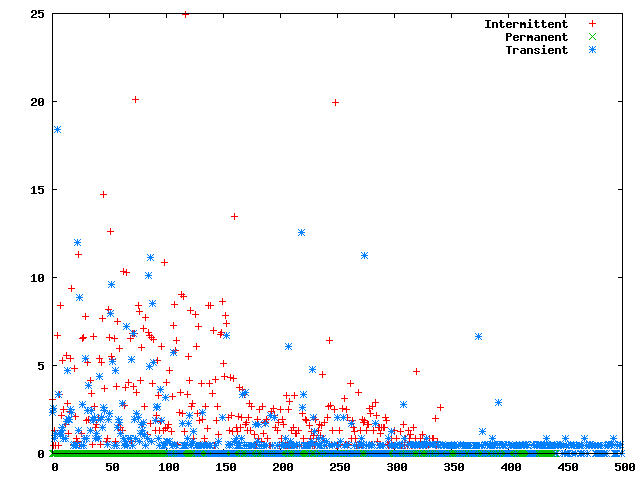
\includegraphics[scale=0.32]{figures/sdsigmap45k.png}
                \caption{Sigma ($\sigma$)}
        \end{subfigure}
        \begin{subfigure}[h]{0.45\linewidth}
                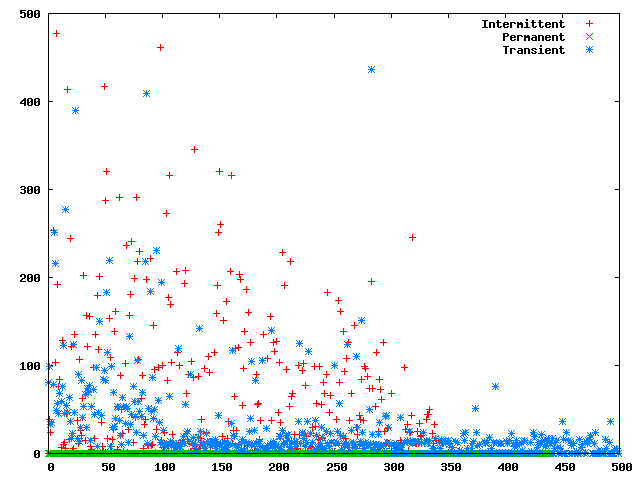
\includegraphics[scale=0.32]{figures/sdiotap45k.png}
                \caption{Iota ($\iota$)}
        \end{subfigure}
			\begin{subfigure}[h]{0.45\linewidth}
                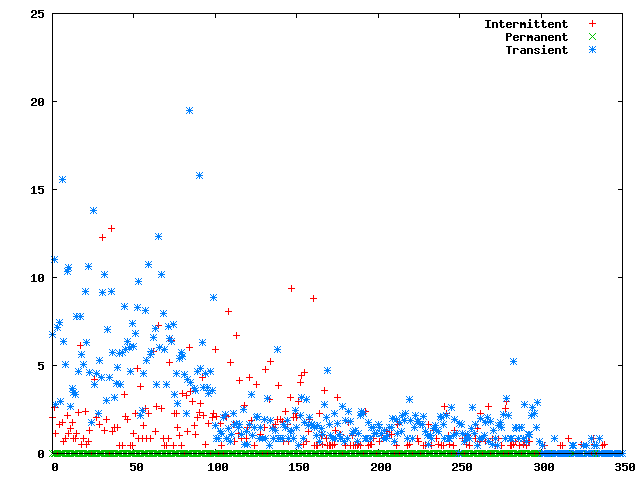
\includegraphics[scale=0.32]{figures/sdtaup45k.png}
                \caption{Tau ($\tau$)}
        \end{subfigure}
        \caption{Standard deviations for evidence-based parameters for p45k}
        \label{fig:sdevidance} 
\end{figure}

Table~\ref{tab:features} summarizes the selected features.
{%
\newcommand{\mc}[3]{\multicolumn{#1}{#2}{#3}}

\captionsetup{justification=centering}
\begin{table}[h]
\begin{tabular}{lll}
\hline
\mc{1}{c}{\textbf{Category}}        & \mc{1}{c}{\textbf{Feature}}       & \mc{1}{c}{\textbf{Symbol}}\\
\hline
\multirow{3}{*}{Non-evidence based features} & Reproducibility of fault                    & $\sigma$\\
                                             & Resemblance of erroneous output patterns  & $\delta_H$\\
                                             & Resemblance of erroneous primary outputs   & $\delta_V$\\
\hline
\multirow{8}{*}{Evidence based features}     & Maximum $\sigma$ among all test runs          & $\sigma$\\
                                             & $\iota$ corresponding to maximum $\sigma$  & $\iota$                             \\
                                             & $\tau$ corresponding to maximum $\sigma$   & $\tau$ \\
                                             & $\gamma$ corresponding to maximum $\sigma$ & $\gamma$ \\
                                             & Standard deviation of $\sigma$             & SD($\sigma$)\\
                                             & Standard deviation of $\iota$              & SD($\iota$)\\
                                             & Standard deviation of $\tau$               & SD($\tau$)\\
                                             & Standard deviation of $\gamma$             & SD($\gamma$)\\
\hline
\end{tabular}
\caption{Summary of selected features}
\label{tab:features}
\end{table}
}%

\section{Selection of machine learning algorithm for fault classification}
\label{sec:selml}

There is a great variety of machine learning algorithms available, and some of the important ones were surveyed in chapter~\ref{chap:chapter3}. The accuracy of the machine learning classifier depends mainly on the complexity of the feature space and actual training data at hand. Now that the feature set is known, the selection of the classifier is done with respect to the following factors:

\begin{description}
  \item[Feature set] The feature set is not statistically independent, an important consideration as it violates the prerequisite for Bayes classifier. It can be seen from plots presented in section~\ref{sec:secfs}, that the feature space has high variance and it is not linearly separable, thus it is not practical to come up with rules to classify faults and hence, the performance of decision trees can be expected to be on the lower side. Also, as the feature space is highly complex, polynomial functions in MLPs might not be sufficient to create an acceptable hypothesis. SVMs, on the other hand can handle kernel functions and can be expected to create a complex hypothesis, as required in our case.

  \item[Sample population] Neural networks and decision trees are known to work well with large training sets \cite{DeFries2000,Tanwani2009}. On the other hand, SVMs are shown to be effective with limited and large sized data sets\cite{Koggalage2004}. In practice, there is no guarantee that a large training dataset will be available before start of manufacturing.
\end{description}

With this, it becomes clear that SVM can be used as classifier of choice as:
\begin{itemize}
  \item SVMs can work well with small and medium size data sets, with relatively high accuracy \cite{Koggalage2004, Matlab2014}.
  \item They can handle n-dimensional feature spaces.
  \item By construction, they can handle complex feature spaces with use of kernel functions.
  \item Once trained, they are fast to classify data .
\end{itemize}
